% Options for packages loaded elsewhere
\PassOptionsToPackage{unicode}{hyperref}
\PassOptionsToPackage{hyphens}{url}
%
\documentclass[
  english,
  man, donotrepeattitle,floatsintext]{apa6}
\usepackage{lmodern}
\usepackage{amssymb,amsmath}
\usepackage{ifxetex,ifluatex}
\ifnum 0\ifxetex 1\fi\ifluatex 1\fi=0 % if pdftex
  \usepackage[T1]{fontenc}
  \usepackage[utf8]{inputenc}
  \usepackage{textcomp} % provide euro and other symbols
\else % if luatex or xetex
  \usepackage{unicode-math}
  \defaultfontfeatures{Scale=MatchLowercase}
  \defaultfontfeatures[\rmfamily]{Ligatures=TeX,Scale=1}
\fi
% Use upquote if available, for straight quotes in verbatim environments
\IfFileExists{upquote.sty}{\usepackage{upquote}}{}
\IfFileExists{microtype.sty}{% use microtype if available
  \usepackage[]{microtype}
  \UseMicrotypeSet[protrusion]{basicmath} % disable protrusion for tt fonts
}{}
\makeatletter
\@ifundefined{KOMAClassName}{% if non-KOMA class
  \IfFileExists{parskip.sty}{%
    \usepackage{parskip}
  }{% else
    \setlength{\parindent}{0pt}
    \setlength{\parskip}{6pt plus 2pt minus 1pt}}
}{% if KOMA class
  \KOMAoptions{parskip=half}}
\makeatother
\usepackage{xcolor}
\IfFileExists{xurl.sty}{\usepackage{xurl}}{} % add URL line breaks if available
\IfFileExists{bookmark.sty}{\usepackage{bookmark}}{\usepackage{hyperref}}
\hypersetup{
  pdflang={en-EN},
  pdfkeywords={NHST, Bayesian, logical fallacy, reanalysis, inner speech, rumination, electromyography},
  hidelinks,
  pdfcreator={LaTeX via pandoc}}
\urlstyle{same} % disable monospaced font for URLs
\usepackage{color}
\usepackage{fancyvrb}
\newcommand{\VerbBar}{|}
\newcommand{\VERB}{\Verb[commandchars=\\\{\}]}
\DefineVerbatimEnvironment{Highlighting}{Verbatim}{commandchars=\\\{\}}
% Add ',fontsize=\small' for more characters per line
\usepackage{framed}
\definecolor{shadecolor}{RGB}{248,248,248}
\newenvironment{Shaded}{\begin{snugshade}}{\end{snugshade}}
\newcommand{\AlertTok}[1]{\textcolor[rgb]{0.94,0.16,0.16}{#1}}
\newcommand{\AnnotationTok}[1]{\textcolor[rgb]{0.56,0.35,0.01}{\textbf{\textit{#1}}}}
\newcommand{\AttributeTok}[1]{\textcolor[rgb]{0.77,0.63,0.00}{#1}}
\newcommand{\BaseNTok}[1]{\textcolor[rgb]{0.00,0.00,0.81}{#1}}
\newcommand{\BuiltInTok}[1]{#1}
\newcommand{\CharTok}[1]{\textcolor[rgb]{0.31,0.60,0.02}{#1}}
\newcommand{\CommentTok}[1]{\textcolor[rgb]{0.56,0.35,0.01}{\textit{#1}}}
\newcommand{\CommentVarTok}[1]{\textcolor[rgb]{0.56,0.35,0.01}{\textbf{\textit{#1}}}}
\newcommand{\ConstantTok}[1]{\textcolor[rgb]{0.00,0.00,0.00}{#1}}
\newcommand{\ControlFlowTok}[1]{\textcolor[rgb]{0.13,0.29,0.53}{\textbf{#1}}}
\newcommand{\DataTypeTok}[1]{\textcolor[rgb]{0.13,0.29,0.53}{#1}}
\newcommand{\DecValTok}[1]{\textcolor[rgb]{0.00,0.00,0.81}{#1}}
\newcommand{\DocumentationTok}[1]{\textcolor[rgb]{0.56,0.35,0.01}{\textbf{\textit{#1}}}}
\newcommand{\ErrorTok}[1]{\textcolor[rgb]{0.64,0.00,0.00}{\textbf{#1}}}
\newcommand{\ExtensionTok}[1]{#1}
\newcommand{\FloatTok}[1]{\textcolor[rgb]{0.00,0.00,0.81}{#1}}
\newcommand{\FunctionTok}[1]{\textcolor[rgb]{0.00,0.00,0.00}{#1}}
\newcommand{\ImportTok}[1]{#1}
\newcommand{\InformationTok}[1]{\textcolor[rgb]{0.56,0.35,0.01}{\textbf{\textit{#1}}}}
\newcommand{\KeywordTok}[1]{\textcolor[rgb]{0.13,0.29,0.53}{\textbf{#1}}}
\newcommand{\NormalTok}[1]{#1}
\newcommand{\OperatorTok}[1]{\textcolor[rgb]{0.81,0.36,0.00}{\textbf{#1}}}
\newcommand{\OtherTok}[1]{\textcolor[rgb]{0.56,0.35,0.01}{#1}}
\newcommand{\PreprocessorTok}[1]{\textcolor[rgb]{0.56,0.35,0.01}{\textit{#1}}}
\newcommand{\RegionMarkerTok}[1]{#1}
\newcommand{\SpecialCharTok}[1]{\textcolor[rgb]{0.00,0.00,0.00}{#1}}
\newcommand{\SpecialStringTok}[1]{\textcolor[rgb]{0.31,0.60,0.02}{#1}}
\newcommand{\StringTok}[1]{\textcolor[rgb]{0.31,0.60,0.02}{#1}}
\newcommand{\VariableTok}[1]{\textcolor[rgb]{0.00,0.00,0.00}{#1}}
\newcommand{\VerbatimStringTok}[1]{\textcolor[rgb]{0.31,0.60,0.02}{#1}}
\newcommand{\WarningTok}[1]{\textcolor[rgb]{0.56,0.35,0.01}{\textbf{\textit{#1}}}}
\usepackage{graphicx}
\makeatletter
\def\maxwidth{\ifdim\Gin@nat@width>\linewidth\linewidth\else\Gin@nat@width\fi}
\def\maxheight{\ifdim\Gin@nat@height>\textheight\textheight\else\Gin@nat@height\fi}
\makeatother
% Scale images if necessary, so that they will not overflow the page
% margins by default, and it is still possible to overwrite the defaults
% using explicit options in \includegraphics[width, height, ...]{}
\setkeys{Gin}{width=\maxwidth,height=\maxheight,keepaspectratio}
% Set default figure placement to htbp
\makeatletter
\def\fps@figure{htbp}
\makeatother
\setlength{\emergencystretch}{3em} % prevent overfull lines
\providecommand{\tightlist}{%
  \setlength{\itemsep}{0pt}\setlength{\parskip}{0pt}}
\setcounter{secnumdepth}{-\maxdimen} % remove section numbering
% Make \paragraph and \subparagraph free-standing
\ifx\paragraph\undefined\else
  \let\oldparagraph\paragraph
  \renewcommand{\paragraph}[1]{\oldparagraph{#1}\mbox{}}
\fi
\ifx\subparagraph\undefined\else
  \let\oldsubparagraph\subparagraph
  \renewcommand{\subparagraph}[1]{\oldsubparagraph{#1}\mbox{}}
\fi
% Manuscript styling
\usepackage{upgreek}
\captionsetup{font=singlespacing,justification=justified}

% Table formatting
\usepackage{longtable}
\usepackage{lscape}
% \usepackage[counterclockwise]{rotating}   % Landscape page setup for large tables
\usepackage{multirow}		% Table styling
\usepackage{tabularx}		% Control Column width
\usepackage[flushleft]{threeparttable}	% Allows for three part tables with a specified notes section
\usepackage{threeparttablex}            % Lets threeparttable work with longtable

% Create new environments so endfloat can handle them
% \newenvironment{ltable}
%   {\begin{landscape}\begin{center}\begin{threeparttable}}
%   {\end{threeparttable}\end{center}\end{landscape}}
\newenvironment{lltable}{\begin{landscape}\begin{center}\begin{ThreePartTable}}{\end{ThreePartTable}\end{center}\end{landscape}}

% Enables adjusting longtable caption width to table width
% Solution found at http://golatex.de/longtable-mit-caption-so-breit-wie-die-tabelle-t15767.html
\makeatletter
\newcommand\LastLTentrywidth{1em}
\newlength\longtablewidth
\setlength{\longtablewidth}{1in}
\newcommand{\getlongtablewidth}{\begingroup \ifcsname LT@\roman{LT@tables}\endcsname \global\longtablewidth=0pt \renewcommand{\LT@entry}[2]{\global\advance\longtablewidth by ##2\relax\gdef\LastLTentrywidth{##2}}\@nameuse{LT@\roman{LT@tables}} \fi \endgroup}

% \setlength{\parindent}{0.5in}
% \setlength{\parskip}{0pt plus 0pt minus 0pt}

% \usepackage{etoolbox}
\makeatletter
\patchcmd{\HyOrg@maketitle}
  {\section{\normalfont\normalsize\abstractname}}
  {\section*{\normalfont\normalsize\abstractname}}
  {}{\typeout{Failed to patch abstract.}}
\makeatother
\shorttitle{The absence of evidence fallacy}
\author{Ladislas Nalborczyk\textsuperscript{1}}
\affiliation{
\vspace{0.5cm}
\textsuperscript{1} Univ. Grenoble Alpes, CNRS, Grenoble INP, GIPSA-lab, 38000 Grenoble, France}
\authornote{

Correspondence concerning this article should be addressed to Ladislas Nalborczyk, GIPSA-lab, CNRS, Univ. Grenoble Alpes, 11 Rue des Mathématiques, 38400 Saint-Martin-d'Hères, France. E-mail: ladislas.nalborczyk@gipsa-lab.fr}
\keywords{NHST, Bayesian, logical fallacy, reanalysis, inner speech, rumination, electromyography}
\usepackage{lineno}

\linenumbers
\usepackage{csquotes}
\ifxetex
  % Load polyglossia as late as possible: uses bidi with RTL langages (e.g. Hebrew, Arabic)
  \usepackage{polyglossia}
  \setmainlanguage[]{english}
\else
  \usepackage[shorthands=off,main=english]{babel}
\fi
\newlength{\cslhangindent}
\setlength{\cslhangindent}{1.5em}
\newenvironment{cslreferences}%
  {\setlength{\parindent}{0pt}%
  \everypar{\setlength{\hangindent}{\cslhangindent}}\ignorespaces}%
  {\par}

\title{\textbf{Submitted to Meta-Psychology. Click here to follow the fully transparent editorial process of this submission. Participate in open peer review by commenting through hypothes.is directly on this preprint.}\\
~\\
~\\
Re-analysing the data from Moffatt et al. (\protect\hyperlink{ref-moffatt_inner_2020}{2020}): A textbook illustration of the absence of evidence fallacy}

\date{}

\abstract{
Moffatt et al. (\protect\hyperlink{ref-moffatt_inner_2020}{2020}) reported the results of an experiment (N = 26 in the final sample) comparing the facial electromyographic correlates of mental rumination and distraction, following an experimentally induced stressor. Based on the absence of significant difference in the perioral muscular activity between the rumination and distraction conditions, Moffatt et al. (\protect\hyperlink{ref-moffatt_inner_2020}{2020}) concluded that \emph{self-reported} inner experience was unrelated to peripheral muscular activity as assessed using surface electromyography. We suggest this conclusion is at best hasty. Indeed, concluding on the absence of an effect based on an under-powered non-significant \emph{p}-value is strongly uninformative. Moreover, the relation between self-reports and physiological measures was not directly assessed, but only indirectly inferred from differences (or absence thereof) in group averages. Given the ample inter-individual variability in these measures (as suggested by our reanalysis), we think inferring the individual-level relation between self-reports and physiological measures from group averages is inappropriate. Given these limitations, we conclude that there is limited evidence for the main conclusion put forward by Moffatt et al. (\protect\hyperlink{ref-moffatt_inner_2020}{2020}) and we suggest ways forward, both from a theoretical and from a methodological perspective. Complete source code, reproducible analyses, and figures are available at \url{https://osf.io/ba3gk/}.
}

\begin{document}
\maketitle

Wordcount (excluding abstract, references, tables, and figures): 4549

\newpage

\hypertarget{introduction}{%
\section{Introduction}\label{introduction}}

The activity of silently talking to oneself or ``inner speech'' is a foundational ability, allowing oneself to remember, plan, self-motivate or self-regulate (for reviews, see Alderson-Day \& Fernyhough, \protect\hyperlink{ref-alderson-day_inner_2015}{2015}; Lœvenbruck et al., \protect\hyperlink{ref-loevenbruck_cognitive_2018}{2018}; Perrone-Bertolotti et al., \protect\hyperlink{ref-perrone-bertolotti_what_2014}{2014}). However, whereas the use inner speech is associated with many adaptive functions in everyday life, inner speech dysfunctions can be identified in multiple psychological disorders. For instance, rumination, broadly defined as unconstructive repetitive thinking about past events and current mood states (Martin \& Tesser, \protect\hyperlink{ref-Martin}{1996}), is involved in the onset and maintenance of serious mental disorders such as depression, anxiety, eating disorders or substance abuse (for a review, see Nolen-Hoeksema et al., \protect\hyperlink{ref-Nolen-Hoeksema2008}{2008}).

Given the predominantly verbal nature of rumination (e.g., Ehring \& Watkins, \protect\hyperlink{ref-ehring_repetitive_2008}{2008}; Goldwin et al., \protect\hyperlink{ref-goldwin_concreteness_2013}{2013}; Goldwin \& Behar, \protect\hyperlink{ref-goldwin_concreteness_2012}{2012}; McLaughlin et al., \protect\hyperlink{ref-mclaughlin_effects_2007}{2007}), we previously proposed to consider rumination as a form of inner speech and to study it using the methods that have been used to study other forms of inner speech, namely, by using surface electromyography and motor interference protocols (e.g., Nalborczyk et al., \protect\hyperlink{ref-nalborczyk_orofacial_2017}{2017}; Nalborczyk, \protect\hyperlink{ref-nalborczyk_understanding_2019}{2019}; Nalborczyk, Perrone-Bertolotti, et al., \protect\hyperlink{ref-nalborczyk_articulatory_2020}{2020}; Nalborczyk, Banjac, et al., \protect\hyperlink{ref-nalborczyk_dissociating_2020}{2020}). We first showed that induced rumination was accompanied by increased facial (both over a forehead and a perioral site) muscular activity in comparison to a rest period (Nalborczyk et al., \protect\hyperlink{ref-nalborczyk_orofacial_2017}{2017}). However, because rumination was only compared to a rest period, it remained uncertain whether this perioral activity was specifically related to (inner) speech processes. Therefore, we ran a follow-up study comparing verbal to non-verbal rumination, which suggested that the facial EMG correlates we have previously identified were not specifically related to the verbal content of the ruminative thoughts (Nalborczyk, Banjac, et al., \protect\hyperlink{ref-nalborczyk_dissociating_2020}{2020}). We discussed these findings in length and proposed several theoretical interpretations that can account for these results in the discussion section of Nalborczyk, Banjac, et al. (\protect\hyperlink{ref-nalborczyk_dissociating_2020}{2020}) and more extensively in Nalborczyk (\protect\hyperlink{ref-nalborczyk_understanding_2019}{2019}). Although these discussions were ignored by Moffatt et al. (\protect\hyperlink{ref-moffatt_inner_2020}{2020}), their experimental design nevertheless had the potential to inform our understanding of the involvement of the speech motor system in different varieties of inner speech as well as to clarify the relation between the peripheral correlates of inner speech and the (self-reported) subjective experience.

The main conclusion from Moffatt et al. (\protect\hyperlink{ref-moffatt_inner_2020}{2020}) is that inner experience between induced rumination and distraction differs ``without a change in electromyographic correlates of inner speech''. In other words, they suggest that the subjective experience of inner speech is unrelated (or loosely related) to the electromyographic correlates of inner speech, which are thought to be represented mostly by the EMG amplitude recorded over the orbicularis oris inferior and orbicularis oris superior muscles. However, for this in-sample observation to be of interest in an out-of-sample context (i.e., to be informative for other non-observed individuals, or said otherwise, to bring information about the population), this absence of difference has to be based on sufficiently powered sample size (given the target effect size) as well as on reliable measures. This is unlikely to be the case here, for reasons that we will present and discuss in the present article. Moreover, a simple visual exploration of the data reveals important variability between individuals in the main effect of interest. That is, some participants had higher perioral muscular activity in the rumination condition than in the distraction condition, and some other participants showed the reverse pattern. This suggests unexplored variation in the determinants of this effect (e.g., the content of the inner experience). Indeed, the relation between the inner experience and the physiological correlates of inner speech production was only inferred from group averages. However, given the important inter-individual variability, this reasoning appears highly problematic. In the following, we explore each of these limitations and suggests ways forward, both from a theoretical and from a methodological perspective.

\hypertarget{exploring-the-data}{%
\section{Exploring the data}\label{exploring-the-data}}

As typical in studies manipulating induced rumination, Moffatt et al. (\protect\hyperlink{ref-moffatt_inner_2020}{2020}) designed a two-step protocol. First, they aimed to induce a negative mood by asking participants to solve unsolvable or excessively difficult anagram and subtraction tasks. Second, they prompted participants to either ruminate on these (purportedly induced) negative feelings (by asking them to ``think about the causes, consequences, and meaning of their current feelings'') or to distract themselves (by asking them to ``think about a village, city or town that you are particularly familiar with''). Rumination and distraction was manipulated within-subject, with all subjects alternating between rumination and distraction, in a counter-balanced order.

Their final sample of participants, after data exclusion, included 26 participants (data available at \url{https://osf.io/hj7tz/}). The EMG data is depicted in Figure \ref{fig:general} by condition (where BAS, DIS, and RUM refer to the baseline, distraction, and rumination conditions, respectively) and by muscle (frontalis, FRO; orbicularis oris inferior, OOI; and orbicularis oris superior, OOS). This figure shows that the average natural logarithm of the EMG peak amplitude recorded over the FRO was at similar levels in the baseline and distraction conditions, but was much higher in the rumination condition. However, the average natural logarithm of the EMG peak amplitude recorded over the OOI and OOS muscles was higher than baseline in both the rumination and distraction conditions, with a slight increase from distraction to rumination (both on the mean and median).

\begin{figure}[!htb]

{\centering 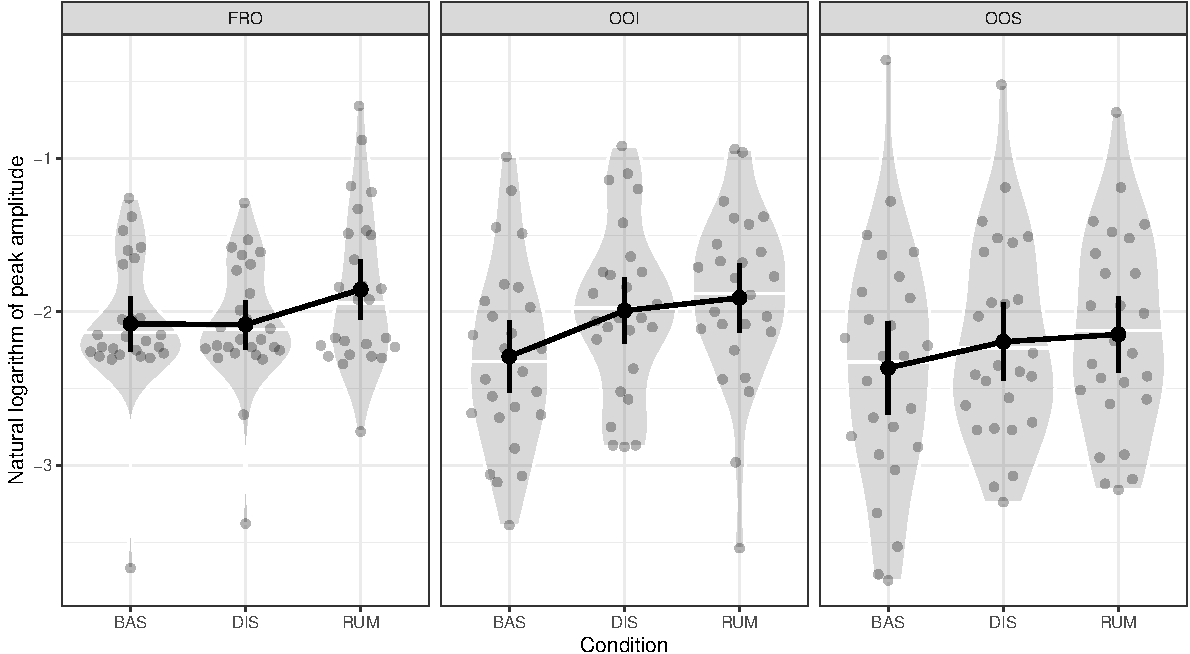
\includegraphics[width=1\linewidth]{manuscript_files/figure-latex/general-1} 

}

\caption{Average natural logarithm of the EMG peak amplitude per muscle and condition. The black dots and intervals represent the by-group average and 95\% confidence interval (N = 26). The horizontal white line in the violin plot represents the median. The grey dots represent the individual-level average natural logarithm of the EMG amplitude by muscle and condition.}\label{fig:general}
\end{figure}

To model EMG peak amplitude variations in response to the rumination and distraction inductions, we fitted a Bayesian multivariate regression model with the natural logarithm of the EMG peak amplitude as an outcome and \emph{Condition} (baseline, rumination, distraction) as a categorical predictor. Therefore, the intercept represents the estimated natural logarithm of the EMG peak amplitude in the baseline condition, and the slopes for the rumination and distraction conditions represent deviations from the baseline. These analyses were conducted using the \texttt{brms} package (Bürkner, \protect\hyperlink{ref-R-brms}{2017}), an \texttt{R} implementation of Bayesian multilevel models that employs the probabilistic programming language \texttt{Stan} (Carpenter et al., \protect\hyperlink{ref-carpenter_stan_2017}{2017}). We ran four chains including each 10.000 iterations and a warmup of 2.000 iterations. Posterior convergence was assessed examining autocorrelation and trace plots, as well as the Gelman-Rubin statistic. Constant effects estimates were summarised via their posterior mean and 95\% credible interval. We also report Bayes factors (BFs) computed using the Savage-Dickey method.\footnote{This method consists in taking the ratio of the posterior density at the point of interest divided by the prior density at that point (Wagenmakers et al., \protect\hyperlink{ref-wagenmakers_bayesian_2010}{2010}).} These BFs can be interpreted as updating factors, from prior knowledge (what we knew before seeing the data) to posterior knowledge (what we know after seeing the data). A summary of the estimations from this model is presented in Table \ref{tab:summary}. This analysis revealed strong evidence for the hypothesis of a higher average EMG peak amplitude in the rumination condition as compared to the baseline condition for both the FRO and OOI muscles (as assessed by the BFs). However, the BFs supported the null hypothesis (i.e., no difference) between the baseline and distraction conditions for the FRO and were inconclusive for both the OOI and OOS muscles.

\begin{table}[H]

\begin{center}
\begin{threeparttable}

\caption{\label{tab:summary}Estimated value of the natural logarithm of the EMG peak amplitude in each condition and for each muscle.}

\small{

\begin{tabular}{lcccccc}
\toprule
Term & \multicolumn{1}{c}{Estimate} & \multicolumn{1}{c}{SE} & \multicolumn{1}{c}{Lower} & \multicolumn{1}{c}{Upper} & \multicolumn{1}{c}{Rhat} & \multicolumn{1}{c}{BF10}\\
\midrule
FRO\_Intercept & -2.076 & 0.096 & -2.266 & -1.888 & 1.000 & 1.785*10\textasciicircum{}16\\
FRO\_conditionDIS & -0.006 & 0.066 & -0.136 & 0.124 & 1.000 & 0.068\\
FRO\_conditionRUM & 0.223 & 0.067 & 0.091 & 0.354 & 1.000 & 19.703\\
OOS\_Intercept & -2.362 & 0.142 & -2.641 & -2.085 & 1.000 & 4.254*10\textasciicircum{}14\\
OOS\_conditionDIS & 0.165 & 0.111 & -0.053 & 0.384 & 1.000 & 0.336\\
OOS\_conditionRUM & 0.212 & 0.111 & -0.005 & 0.432 & 1.000 & 0.689\\
OOI\_Intercept & -2.284 & 0.117 & -2.514 & -2.053 & 1.001 & 7.411*10\textasciicircum{}15\\
OOI\_conditionDIS & 0.290 & 0.120 & 0.054 & 0.526 & 1.000 & 2.006\\
OOI\_conditionRUM & 0.371 & 0.119 & 0.137 & 0.603 & 1.000 & 12.876\\
\bottomrule
\addlinespace
\end{tabular}

}

\begin{tablenotes}[para]
\normalsize{\textit{Note.} For each effect, the 'Estimate' reports the estimated average value of the natural logarithm of the EMG peak amplitude, followed by its standard error (SE). The 'Lower' and 'Upper' columns contain the lower and upper bounds of the 95\% CrI, whereas the 'Rhat' column reports the Gelman-Rubin statistic. The last column reports the BF in favour of the alternative hypothesis (relative to the null hypothesis).}
\end{tablenotes}

\end{threeparttable}
\end{center}

\end{table}

Because the result of a Bayesian analysis is a joint posterior probability over all parameters of the model, we can compute the posterior distribution of the difference between any pair of conditions. In Figure \ref{fig:posterior} we represent the posterior distribution of the difference in EMG peak amplitude between the rumination and distraction condition for each muscle. This figure reveals that the most probable value for this difference was \(\beta = 0.228\) (95\% CrI {[}0.098, 0.357{]}) for the FRO muscle, \(\beta = 0.081\) (95\% CrI {[}-0.155, 0.324{]}) for the FRO muscle, and \(\beta = 0.047\) (95\% CrI {[}-0.167, 0.27{]}) for the OOS muscle. Moreover, comparing the posterior distribution to \(\theta = 0\) reveals that there is a probability of 0.753 that the average peak EMG amplitude recorded over the OOI is higher in the rumination condition than in the distraction condition (given the model, the priors, and the data from Moffatt et al., \protect\hyperlink{ref-moffatt_inner_2020}{2020}).

\begin{figure}[!htb]

{\centering 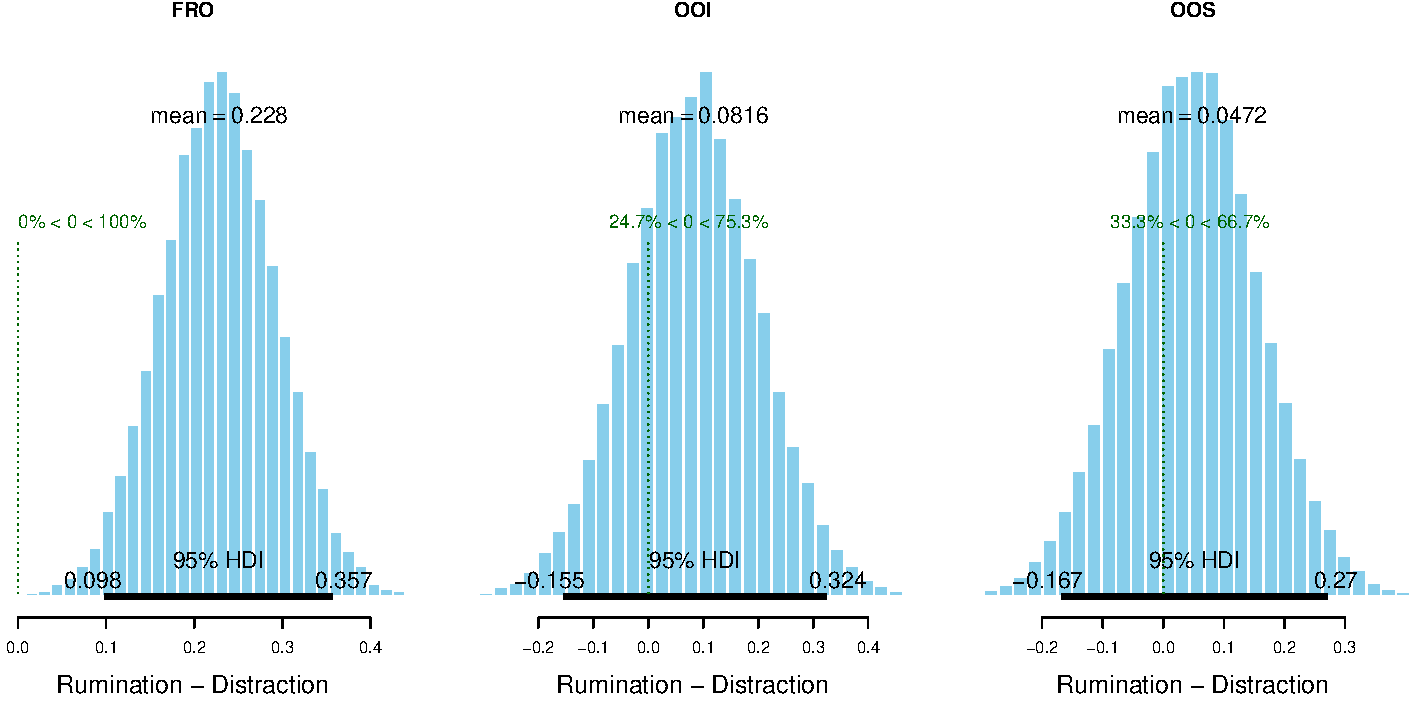
\includegraphics[width=1\linewidth]{manuscript_files/figure-latex/posterior-1} 

}

\caption{Posterior distribution of the difference in EMG peak amplitude between the rumination and distraction condition for each muscle, along with its mean and 95\% credible interval.}\label{fig:posterior}
\end{figure}

Having nuanced some of the conclusions from Moffatt et al. (\protect\hyperlink{ref-moffatt_inner_2020}{2020}), we now turn to a discussion of the problems related to conclusions that can be made from under-powered non-significant results.

\hypertarget{concluding-on-the-null-hypothesis-from-under-powered-null-hypothesis-significance-tests-what-could-possibly-go-wrong}{%
\subsection{Concluding on the null hypothesis from under-powered null-hypothesis significance tests: what could possibly go wrong?}\label{concluding-on-the-null-hypothesis-from-under-powered-null-hypothesis-significance-tests-what-could-possibly-go-wrong}}

There is an infamous tradition of conducting and interpreting uninformative null-hypothesis significance tests in Psychology (e.g., Meehl, \protect\hyperlink{ref-harlow_problem_1997}{1997}, \protect\hyperlink{ref-meehl_theoretical_1978}{1978}, \protect\hyperlink{ref-meehl_why_1990}{1990}\protect\hyperlink{ref-meehl_why_1990}{a}, \protect\hyperlink{ref-meehl_appraising_1990-1}{1990}\protect\hyperlink{ref-meehl_appraising_1990-1}{b}, \protect\hyperlink{ref-meehl_theory-testing_1967}{1967}). By ``uninformative'', we mean that some null-hypothesis significance tests are simply not diagnostic with regards to the substantive effect of interest (e.g., whether there is a difference between conditions A and B).

As highlighted by several authors (e.g., Cohen, \protect\hyperlink{ref-cohen_earth_1994}{1994}; Pollard \& Richardson, \protect\hyperlink{ref-pollard_probability_1987}{1987}; Rouder et al., \protect\hyperlink{ref-rouder_is_2016}{2016}), concluding that an effect is probably absent solely based on a non-significant \emph{p}-value is the continuous (i.e., probabilistic) extension of the modus tollens and is not a valid argument (i.e., the conclusion does not follow from the premises). This fallacious argument is also known as the \emph{fallacy of acceptance}, the \emph{absence of evidence fallacy} or \emph{the argument from ignorance}, and proceeds as follows: ``If the null hypothesis is true, then this observation should \emph{rarely} occur. This observation occurred. Therefore, the null hypothesis is false (or has low probability)''. In short, this argument is fallacious because it fails to consider the alternative hypothesis.

This problem is tackled in modern usages of null-hypothesis significance tests by ensuring that the claim under scrutiny is submitted to \emph{severe} tests (e.g., Mayo \& Spanos, \protect\hyperlink{ref-mayo_severe_2006}{2006}; Mayo, \protect\hyperlink{ref-mayo_statistical_2018}{2018}). In general terms, the strong severity principle states that we have evidence for a claim to the extent that it survives a stringent scrutiny, that is, to the extent that it survives \emph{severe} tests. More precisely, some claim (e.g., \(\theta = 0\)) is said to be \emph{severely tested} if it had great chances of being falsified, had the claim been false. When a statistical test is under-powered (for detecting a given effect size), the claim under scrutiny is not strongly (severely) tested, hence it not possible to obtain strong or reliable evidence for the claim (bad test, no evidence).

Anticipating the legitimate critiques on the power of their study, Moffatt et al. (\protect\hyperlink{ref-moffatt_inner_2020}{2020}) report the results of a power analysis using the effect size reported in Nalborczyk et al. (\protect\hyperlink{ref-nalborczyk_orofacial_2017}{2017}) of \(d = 0.72\). This represents a highly optimistic estimate of the substantive effect of interest (i.e., the difference in the natural logarithm of the EMG peak amplitude between the rumination and distraction conditions) as this effect represents the standardised mean difference in EMG amplitude \emph{between a rest and a rumination periods} (Nalborczyk et al., \protect\hyperlink{ref-nalborczyk_orofacial_2017}{2017}).

We suggest the (a priori) power of the study ran by Moffatt et al. (\protect\hyperlink{ref-moffatt_inner_2020}{2020}) was much lower than suggested by the authors. Indeed, we speculate that the standardised mean difference in EMG peak amplitude between the rumination and distraction conditions may be much weaker than the standardised mean difference in EMG amplitude between the rumination and rest conditions. If we assume that the former is half the size of the latter (which seems reasonable given the high inter-individual variability in such effects, cf.~the next section but also Nalborczyk, Grandchamp, et al., \protect\hyperlink{ref-nalborczyk_can_2020}{2020}), therefore the a priori power of the main statistical test from Moffatt et al. (\protect\hyperlink{ref-moffatt_inner_2020}{2020}) was around \(0.42\), meaning that they had less than 1 chance out of 2 to find a significant effect (given that the population effect size was actually \(0.36\)).

\begin{Shaded}
\begin{Highlighting}[]
\CommentTok{\# A priori power for n = 26 and d = 0.36}
\KeywordTok{library}\NormalTok{(pwr)}
\KeywordTok{pwr.t.test}\NormalTok{(}
  \DataTypeTok{n =} \DecValTok{26}\NormalTok{, }\DataTypeTok{d =} \FloatTok{0.72} \OperatorTok{/}\StringTok{ }\DecValTok{2}\NormalTok{, }\DataTypeTok{sig.level =} \FloatTok{0.05}\NormalTok{,}
  \DataTypeTok{type =} \StringTok{"one.sample"}\NormalTok{, }\DataTypeTok{alternative =} \StringTok{"two.sided"}
\NormalTok{  )}
\end{Highlighting}
\end{Shaded}

\begin{verbatim}
## 
##      One-sample t test power calculation 
## 
##               n = 26
##               d = 0.36
##       sig.level = 0.05
##           power = 0.4228455
##     alternative = two.sided
\end{verbatim}

Once again, anticipating the legitimate critique that the absence of a significant difference is not necessarily ``significant'' evidence for the absence of an effect, Moffatt et al. (\protect\hyperlink{ref-moffatt_inner_2020}{2020}) reported the following Bayes factor (BF) analysis:

\begin{quote}
``{[}\ldots{]} therefore it is possible that the sample size of the present study lacked sufficient power to detect the effect of rumination on muscle activity. In order to test this, a Bayesian paired samples t-test was conducted for the peak log values of muscle activity between the rumination and distraction conditions. This revealed strong evidence in favour of the alternative hypothesis for the FRO muscle (\(B_{10} = 18.79\)), and moderate evidence in favour of the null hypothesis for the OOS (\(B_{10} = 0.232\)) and OOI (\(B_{10} = 0.278\)) muscles, according to current guidelines for interpreting Bayes factors {[}43{]}.''
\end{quote}

While we appreciate the effort, the current approach poses new problems. First, contrary to what the authors suggest, whereas computing a BF indeed allows assessing the \emph{relative evidence} for the null, computing a BF (i.e., comparing two models) does not solve at all the problem of low power. More precisely, the sensitivity (i.e., the ability to attain a certain goal) of an experimental design to detect a given effect is an issue for both frequentist and Bayesian statistical tests. To illustrate this point, we present below the results of two simulations.

\begin{figure}[!htb]

{\centering 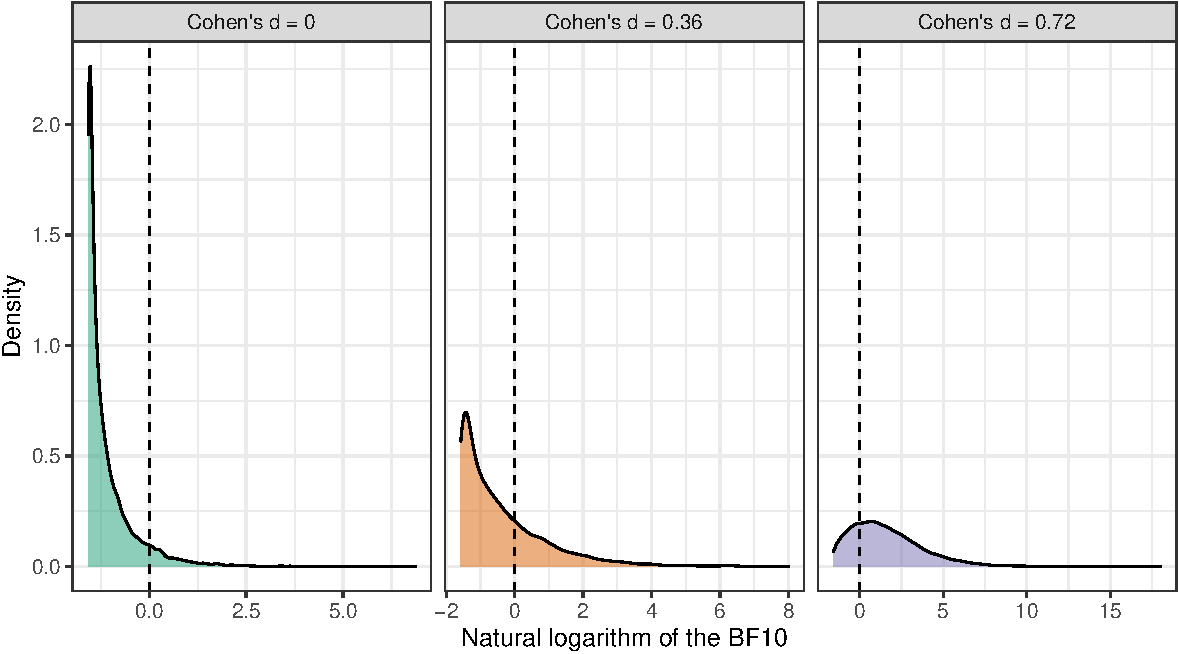
\includegraphics[width=1\linewidth]{manuscript_files/figure-latex/bf-dance-1} 

}

\caption{Illustrating the distribution of Bayes factors in favour of the alternative hypothesis for different population effect sizes (N = 26). In the left panel, the effect size is fixed to d = 0 (i.e., the null hypothesis), in the middle panel, it is fixed to d = 0.36 (i.e., the supposed target effect size in Moffatt et al., 2020), and in the right panel, the effect size is fixed to d = 0.72 (i.e., the effect size reported in Nalborczyk et al., 2017).}\label{fig:bf-dance}
\end{figure}

First, we simulated 10.000 datasets (for \(N = 26\)) under the assumption of either no effect (i.e., the null hypothesis of \(d = 0\)), an effect size of \(d = 0.36\) (i.e., the supposed target effect size in Moffatt et al., \protect\hyperlink{ref-moffatt_inner_2020}{2020}), or an effect size of \(d = 0.72\) (i.e., the effect size reported in Nalborczyk et al., \protect\hyperlink{ref-nalborczyk_orofacial_2017}{2017}). As shown in Figure \ref{fig:bf-dance}, the distribution of BFs computed under each hypothesis reveals important inter-simulation variability. For instance, under the null hypothesis, 6.96\% of the computed BFs are above 0 and hence support the alternative hypothesis (although the ``true'' effect size is \(d = 0\)). When the ``true'' effect size is of \(d = 0.36\), 71.83\% of the BFs are below 0 and hence support the null hypothesis (although the true effect size is actually non-null). When the ``true'' effect size is of \(d = 0.72\), 25.58\% of the BFs are still below 0. In other words, for small sample and effect sizes, BFs have high error rates.\footnote{To assess the extent to which the \(\text{BF}_{10}\) computed for the OOI by Moffatt et al. (\protect\hyperlink{ref-moffatt_inner_2020}{2020}) is ``surprising'' given or ``compatible'' with the hypothesis of an effect size of \(d = 0.36\), we can compute the probability of obtaining this finding or a more extreme finding given the hypothesis, which is approximately equal to 0.29.}

Second, we conducted another simulation with the aim of assessing the relation between the sample size and the value of the BF. In the previous section, we fitted a multivariate Bayesian regression model with varying-intercepts by participant and weakly informative priors on the EMG data collected by Moffatt et al. (\protect\hyperlink{ref-moffatt_inner_2020}{2020}). Using this model, we i) generated new datasets from the posterior predictive distribution of this model and ii) we computed the BF in favour of the alternative hypothesis (\(\text{BF}_{10}\)) using the \texttt{BayesFactor} package (Morey \& Rouder, \protect\hyperlink{ref-R-BayesFactor}{2018}). We used a ``medium'' prior (i.e., \(r = \sqrt{2}/2\)) on the scale of the Cauchy prior for the alternative hypothesis. We repeated this procedure for varying sample sizes from 20 to 200 participants (by increments of 10 participants) with \(1000\) simulations (i.e., 1000 simulated datasets) for each sample size.

\begin{figure}[!htb]

{\centering 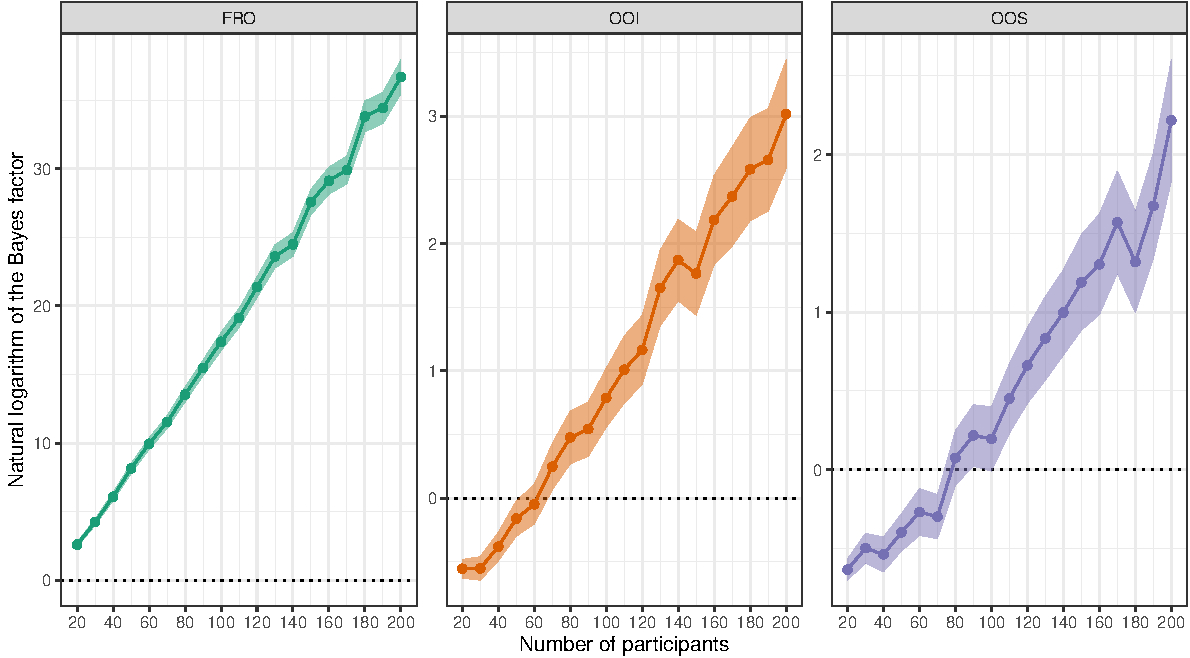
\includegraphics[width=1\linewidth]{manuscript_files/figure-latex/simulated-power-1} 

}

\caption{Average natural logarithm of the Bayes factor in favour of the alternative hypothesis, along with its standard error, computed over 1000 datasets of increasing size simulated from the posterior predictive distribution of the varying-intercept multivariate Bayesian regresion model, fitted on the data from Moffatt et al. (2020). A log-BF belows 0 represents evidence for the null hypothesis (relative to the alternative hypothesis) and a log-BF above 0 represents evidence for the alternative hypothesis (relative to the null hypothesis).}\label{fig:simulated-power}
\end{figure}

As shown in Figure \ref{fig:simulated-power}, the natural logarithm of the BF in favour of the alternative hypothesis is growing proportionally with sample size. More precisely, whereas BFs computed on small samples (i.e., below 80 participants) support the null hypothesis, BFs computed on larger samples support the alternative hypothesis for all three facial muscles. For instance, the average \(\text{BF}_{10}\) computed for the OOI muscle with a sample size of 160 participants is of \(\exp(2.18) \approx 8.85\), indicating that these data are approximately \(8.85\) times more likely under the alternative hypothesis than under the null hypothesis. To sum up, this reveals that although at low sample sizes, the BF may provide (weak) evidence for the null hypothesis (relative to the alternative hypothesis), this pattern may very well reverse for higher sample sizes.

We should keep in mind some limitations of this analysis, which uses simulated datasets form the posterior predictive distribution estimated on the data collected by Moffatt et al. (\protect\hyperlink{ref-moffatt_inner_2020}{2020}). This analysis resembles to the Bayesian analogue of the frequentist post-hoc power analysis, which has been much criticised (e.g., Lakens, \protect\hyperlink{ref-lakens_20_2014}{2014}). A crucial assumption of the present analysis is that the data from Moffatt et al. (\protect\hyperlink{ref-moffatt_inner_2020}{2020}) is our best source of information regarding the main effect of interest. However, the present analysis also differs from the frequentist post-hoc power analysis on several grounds. First, with the present analysis, we do not aim to assess the ability of our statistical test to pass some dichotomic threshold (e.g., accept/reject). Instead, we aim to assess how the \(\text{BF}_{10}\) (i.e., the evidence for the alternative hypothesis, relative to the null hypothesis) behaves with varying sample sizes. Second, the present analysis relies on the posterior predictive distribution of the model fitted on the data from Moffatt et al. (\protect\hyperlink{ref-moffatt_inner_2020}{2020}), which naturally incorporates uncertainty about the effect of interest. By simulating datasets of varying sample sizes from the posterior predictive distribution (and by relying on a large number of simulations), uncertainty about the effect size is naturally incorporated into the results of the simulation.

\hypertarget{within-subject-manipulation-of-rumination-and-distraction}{%
\subsection{Within-subject manipulation of rumination and distraction}\label{within-subject-manipulation-of-rumination-and-distraction}}

In Nalborczyk, Banjac, et al. (\protect\hyperlink{ref-nalborczyk_dissociating_2020}{2020}), we manipulated the modality of rumination (whether it is verbal or non-verbal) in a between-subject manner to avoid order effects and to avoid dissipating the effects of the negative mood induction. More precisely, we assumed that inducing rumination after a distraction condition in a within-subject manner would dissipate the effects of the mood induction and therefore reduce the impact of the rumination induction. In contrast to this approach, Moffatt et al. (\protect\hyperlink{ref-moffatt_inner_2020}{2020}) asked participants to ruminate and then distract themselves (or reciprocally), after an induced stressor (an induced failure). In Figure \ref{fig:order}, we depict again the EMG data, this time grouped by the order in which the participants went through the rumination and distraction conditions. This figure reveals some potentially interesting differences between the two groups of participants. For instance, the participants that first went through the rumination condition (in green) seem to show a higher increase in the average EMG peak amplitude recorded over the FRO muscle from baseline than the participants that first went through the distraction condition (in orange).

\begin{figure}[!htb]

{\centering 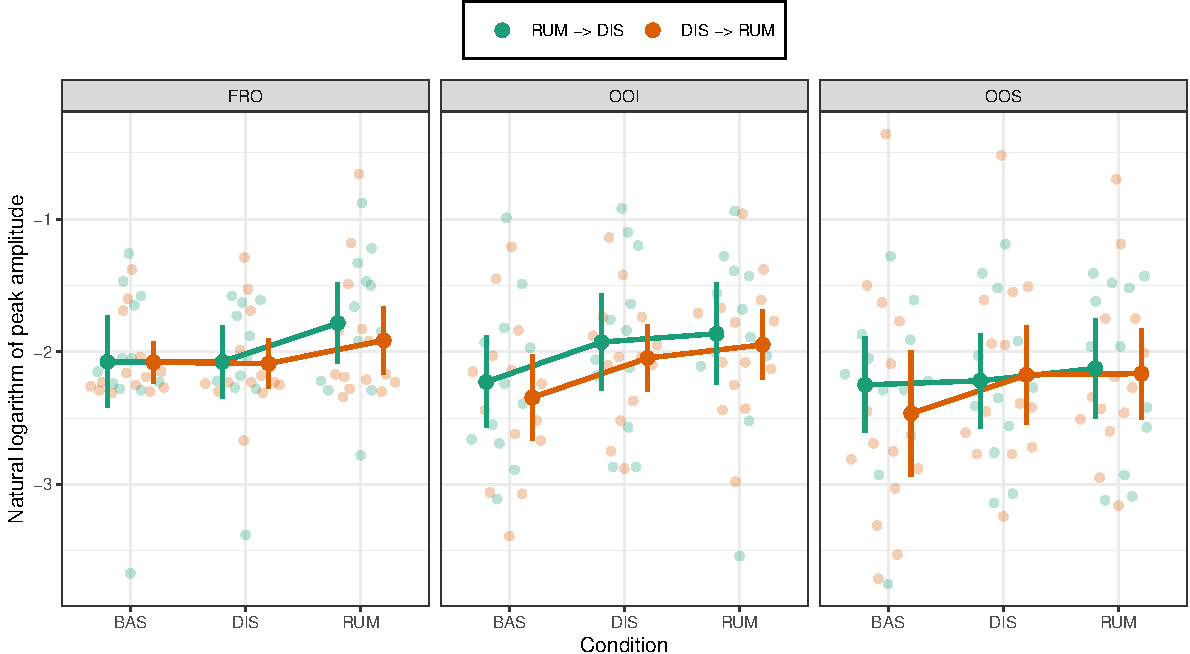
\includegraphics[width=1\linewidth]{manuscript_files/figure-latex/order-1} 

}

\caption{Average natural logarithm of the EMG peak amplitude by muscle, condition, and group. The green dots and intervals represent the by-group average and 95\% confidence interval for the participants that first went through the rumination condition, then through the distraction condition. The orange dots and intervals represent the by-group average and 95\% confidence interval for the participants that first went through the distraction condition, then through the rumination condition. The light green and orange dots in the background represent the individual-level average natural logarithm of the EMG amplitude by muscle, condition, and group.}\label{fig:order}
\end{figure}

Anticipating again that the order of the within-subject conditions may be an issue, Moffatt et al. (\protect\hyperlink{ref-moffatt_inner_2020}{2020}) say:

\begin{quote}
``Unless otherwise reported, the inclusion of order in which the conditions were completed as a between-subjects variable as part of a mixed-design ANOVA produced no significant main effects or interactions involving order.''
\end{quote}

Unfortunately, the problems we discussed in the previous section about the interpretation of under-powered non-significant results also apply to this test. Namely, obtaining a non-significant effect of group is very weak evidence that order did not play a role in the results, given the low power of the tests that were performed. This statistical argument is supported by the visual exploration of the data presented in Figure \ref{fig:order}, which suggests possibly crucial differences between the two groups of participants. However, given the sample size in each group (N = 12 and N = 14), it is impossible to know for sure at this point.

\hypertarget{does-everyone-show-the-effect}{%
\subsection{Does everyone show the effect?}\label{does-everyone-show-the-effect}}

We previously noted (e.g., Nalborczyk et al., \protect\hyperlink{ref-nalborczyk_orofacial_2017}{2017}; Nalborczyk, \protect\hyperlink{ref-nalborczyk_understanding_2019}{2019}; Nalborczyk, Banjac, et al., \protect\hyperlink{ref-nalborczyk_dissociating_2020}{2020}; Nalborczyk, Grandchamp, et al., \protect\hyperlink{ref-nalborczyk_can_2020}{2020}) that surface EMG measures of inner speech production were highly variable between individuals. This can be explained by the imagery ability of each individual, the reliability of the measurement, and the instructions that are given to the participants (and whether they are understood in a similar manner by all participants). The data collected by Moffatt et al. (\protect\hyperlink{ref-moffatt_inner_2020}{2020}) is no exception and presents an important degree of inter-individual variability. In Figure \ref{fig:everyone}, we represent again the EMG data for each participant (each line is a participant). We used two colours to represent the participants that showed a higher average EMG peak amplitude either in the rumination condition (in green) or in the distraction condition (in orange). As it can be seen from this figure, whereas some participants show ``intermediate'' or ``ambiguous'' (i.e., equivalent) patterns of muscular activity across conditions, some participants show a clear superior EMG peak amplitude in the rumination condition (in green) and some others in the distraction condition (in orange).

\begin{figure}[!htb]

{\centering 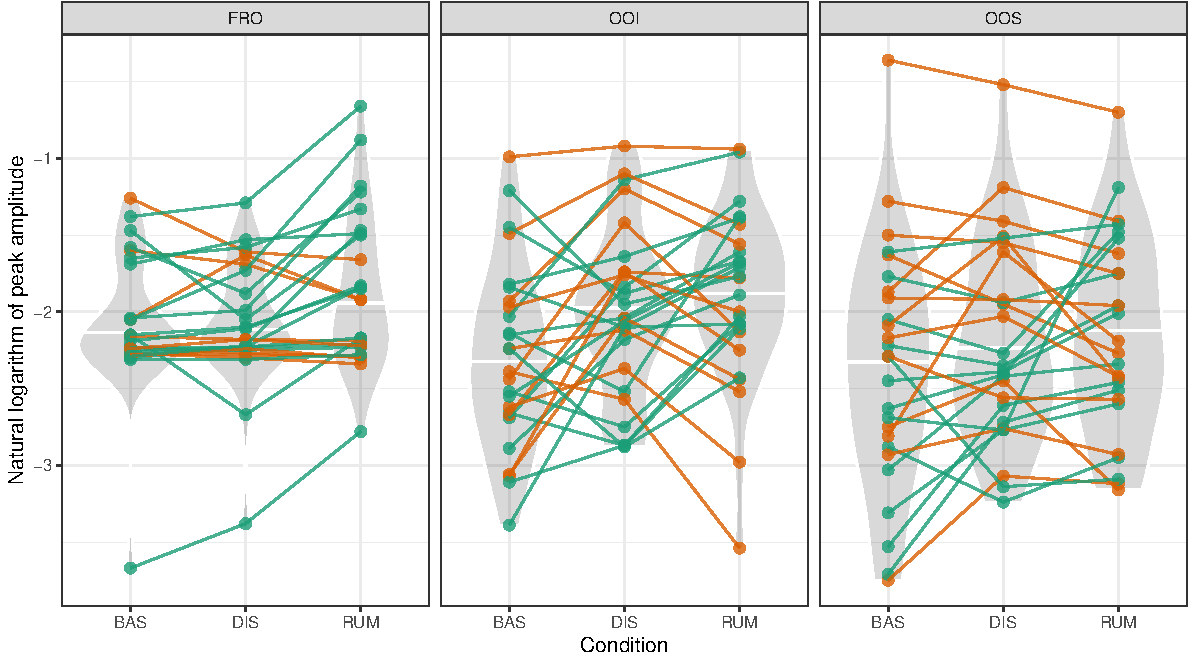
\includegraphics[width=1\linewidth]{manuscript_files/figure-latex/everyone-1} 

}

\caption{Inter-individual variability in the main effect of interest (i.e., the difference between the rumination and distraction conditions). Green dots and lines represent the average natural logarithm of the EMG amplitude of participants that showed a higher EMG amplitude in the rumination condition than in the distraction condition, whereas orange dots and lines represent the average natural logarithm of the EMG amplitude of participants that showed a higher EMG amplitude in the distraction condition than in the rumination condition.}\label{fig:everyone}
\end{figure}

This important inter-individual variability calls into question the use of group averages to describe the nature of inner speech at an individual level. Moreover, this variability suggests that some important confounding factors were not taken into account (i.e., either not manipulated in the experiment or statistically controlled for). In line with Moffatt et al. (\protect\hyperlink{ref-moffatt_inner_2020}{2020}), we suggest these discrepancies could be explained by differences in the subjective experience of inner speech. We agree that a lot could be learnt by relating this (self-reported) subjective experience to the peripheral muscular correlates of inner speech production. However, this can not be done at the group level, at the risk of missing individual-level patterns. Therefore, we encourage Moffatt et al. (\protect\hyperlink{ref-moffatt_inner_2020}{2020}) to analyse further their data in order to assess whether the perioral EMG correlates (e.g., the amplitude of the difference between the rumination and distraction conditions on the OOI) can be predicted by the self-reported subjective experience, \emph{at an individual level}.

It should be noted that the question of the qualitative differences in the EMG correlates of inner speech may also be assessed more formally using the model comparison approach developed by Haaf and Rouder (\protect\hyperlink{ref-haaf_developing_2017}{2017}). However, this would require data coming from an experimental design in which inner speech and non-inner speech conditions would be manipulated within-subject and with multiple observations for each participants in each condition (e.g., as in Nalborczyk, Grandchamp, et al., \protect\hyperlink{ref-nalborczyk_can_2020}{2020}).

\hypertarget{discussion-and-conclusions}{%
\section{Discussion and conclusions}\label{discussion-and-conclusions}}

With this paper we aimed to nuance the strong conclusion made by Moffatt et al. (\protect\hyperlink{ref-moffatt_inner_2020}{2020}), who asserted that the inner experience of rumination was not related to its peripheral muscular correlates. First, we reanalysed the data from Moffatt et al. (\protect\hyperlink{ref-moffatt_inner_2020}{2020}) and provided some nuance to the conclusion that can be made from these data. Second, we discussed the statistical and epistemological reasons that cast doubt upon the main conclusion of Moffatt et al. (\protect\hyperlink{ref-moffatt_inner_2020}{2020}). Because the tests conducted by Moffatt et al. (\protect\hyperlink{ref-moffatt_inner_2020}{2020}) were heavily under-powered, they provide only weak evidence for the absence of difference. Third, we highlighted that the order of the conditions participants went through may impact the effects of the rumination induction (although we can not decide on this issue with the present data). Finally, we showed that the group analyses masked important inter-individual variability that should be more carefully examined.

In addition to these methodological limitations, we now wish to discuss the theoretical interpretations and implications of these results. As discussed in the introduction section, we previously conducted several studies aiming to assess the role of the speech motor system in rumination. Following our initial study (Nalborczyk et al., \protect\hyperlink{ref-nalborczyk_orofacial_2017}{2017}), we ran an extension in which we compared verbal to non-verbal rumination. The results suggested that the facial EMG correlates of verbal and non-verbal rumination were similar (Nalborczyk, Banjac, et al., \protect\hyperlink{ref-nalborczyk_dissociating_2020}{2020}). Given the ample evidence on the EMG correlates of inner speech production (for an overview, see Chapter 1 in Nalborczyk, \protect\hyperlink{ref-nalborczyk_understanding_2019}{2019}), we needed to explain why this particular form of inner speech (induced rumination) was not associated with speech-specific peripheral muscular activity.

In Nalborczyk, Banjac, et al. (\protect\hyperlink{ref-nalborczyk_dissociating_2020}{2020}), we suggested that this observation was coherent with the mental-habit view of depressive rumination (Watkins \& Nolen-Hoeksema, \protect\hyperlink{ref-watkins_habit-goal_2014}{2014}), which defines rumination as a habitual behaviour, automatically triggered by contextual cues such as negative mood. We know habitual behaviours are more automatic (they are not intentionally initiated) than non-habitual behaviours. Interestingly, it has been observed that the automaticity with which a verbal thought is evoked may influence the degree to which it is enacted, that is, the degree to which it recruits the speech motor system (e.g., Cohen, \protect\hyperlink{ref-cohen_motor_1986}{1986}; Sokolov, \protect\hyperlink{ref-sokolov_inner_1972}{1972}). According to Cohen (\protect\hyperlink{ref-cohen_motor_1986}{1986}), the presence of peripheral motor activity during inner speech production may be interpreted in terms of attention sharing. For instance, in novel (hence non-automatic) or difficult situations, the vividness of inner speech may be strengthened by increasing the speech motor activity, resulting in more salient auditory percepts. Relating this idea to the motor control framework we previously proposed (e.g., Lœvenbruck et al., \protect\hyperlink{ref-loevenbruck_cognitive_2018}{2018}; Grandchamp et al., \protect\hyperlink{ref-grandchamp_condialint_2019}{2019}), it may be said that the characteristics of the situation (e.g., novelty, difficulty) may influence the amount of inhibition that is applied to motor commands during inner speech production, hence resulting in more or less visible peripheral muscular activity (see also a discussion of theses ideas in the broader context of motor imagery, Guillot et al., \protect\hyperlink{ref-guillot_imagining_2012}{2012}).

Another possible interpretation is that automatic forms of inner speech may rely more heavily on higher-level (e.g., memory-based) cognitive processes whereas less automatic (i.e., more intentional or deliberate) forms of inner speech may rely more on simulation mechanisms via the use of internal models of the speech motor systems (Nalborczyk, \protect\hyperlink{ref-nalborczyk_understanding_2019}{2019}). In other words, the production of automatic or non-automatic inner speech would be underpinned by different processes that would involve the speech motor system to a different extent. This distinction is similar to the distinction between the two routes of predictions-by-association and prediction-by-simulations in speech perception and comprehension (Pickering \& Garrod, \protect\hyperlink{ref-pickering_integrated_2013}{2013}). The prediction-by-association mechanism would rely more on perceptual sensory experiences and domain-general cognitive abilities whereas the prediction-by-simulation mechanism would rely more simulation of the motor action leading to the speech auditory percept. In the former case, no peripheral muscular activity is expected, whereas in the latter case, the speech motor system would be involved in simulating/emulating the corresponding overt action (cf.~also the motor simulation vs.~direct simulation (memory retrieval) distinction in Tian \& Poeppel, \protect\hyperlink{ref-tian_mental_2012}{2012}). Whether the physiological correlates of automatic and non-automatic (deliberate) forms of inner speech differ because of inhibitory constraints or because they rely on different processes (e.g., prediction-by-association or prediction-by-simulation) remains an open empirical question. We previously discussed these issues in more length and suggested ways forward from an experimental perspective (cf.~the discussion in Nalborczyk, \protect\hyperlink{ref-nalborczyk_understanding_2019}{2019}).

To conclude, we wish to bring some nuance to the conclusion of Moffatt et al. (\protect\hyperlink{ref-moffatt_inner_2020}{2020}), who stated that ``In conclusion, induced rumination appeared to involve similar levels of inner speech-related muscle activity to a period of distraction''. In consideration of the limitations discussed in the present article, this conclusion seems hasty. Indeed, we provided theoretical (epistemological) and empirical (via simulation) reasons to doubt the strength of the evidence for the null hypothesis in this study. Moreover, supplementary analyses showed that the order of the conditions participants went through may have influenced the effects of the rumination induction on the EMG correlates. Finally, important under-explored inter-individual variability suggests that important determinants of these correlates were not taken into account. We urge the authors to nuance their conclusions, to analyse further their data, and to plan adequately-powered studies in order to settle these issues.

\hypertarget{supp}{%
\section{Supplementary materials}\label{supp}}

Reproducible code and figures are available at \url{https://osf.io/ba3gk/}.

\hypertarget{acknowledgements}{%
\section*{Acknowledgements}\label{acknowledgements}}
\addcontentsline{toc}{section}{Acknowledgements}

We thank Antonio Schettino for suggesting to include the ``Dance of the Bayes factors'' simulation and for provding helpful comments on a previous version of this manuscript.

\hypertarget{references}{%
\section*{References}\label{references}}
\addcontentsline{toc}{section}{References}

\hypertarget{refs}{}
\begin{cslreferences}
\leavevmode\hypertarget{ref-alderson-day_inner_2015}{}%
Alderson-Day, B., \& Fernyhough, C. (2015). Inner speech: Development, cognitive functions, phenomenology, and neurobiology. \emph{Psychological Bulletin}, \emph{141}(5), 931--965. \url{https://doi.org/10.1037/bul0000021}

\leavevmode\hypertarget{ref-R-papaja}{}%
Aust, F., \& Barth, M. (2017). \emph{papaja: Create APA manuscripts with R Markdown}. \url{https://github.com/crsh/papaja}

\leavevmode\hypertarget{ref-R-brms}{}%
Bürkner, P.-C. (2017). brms: An R package for bayesian multilevel models using Stan. \emph{Journal of Statistical Software}, \emph{80}(1), 1--28. \url{https://doi.org/10.18637/jss.v080.i01}

\leavevmode\hypertarget{ref-carpenter_stan_2017}{}%
Carpenter, B., Gelman, A., Hoffman, M., Lee, D., Goodrich, B., Betancourt, M., Brubaker, M., Guo, J., Li, P., \& Riddell, A. (2017). Stan: A probabilistic programming language. \emph{Journal of Statistical Software, Articles}, \emph{76}(1), 1--32. \url{https://doi.org/10.18637/jss.v076.i01}

\leavevmode\hypertarget{ref-cohen_motor_1986}{}%
Cohen, B. H. (1986). The motor theory of voluntary thinking. In R. J. Davidson, G. E. Schartz, \& D. Shapiro (Eds.), \emph{Consciousness and self-regulation}. Springer, Boston, MA.

\leavevmode\hypertarget{ref-cohen_earth_1994}{}%
Cohen, J. (1994). The earth is round (p \(<\) .05). \emph{American Psychologist}, \emph{49}(12), 997--1003. \url{https://doi.org/10.1037/0003-066X.49.12.997}

\leavevmode\hypertarget{ref-ehring_repetitive_2008}{}%
Ehring, T., \& Watkins, E. R. (2008). Repetitive negative thinking as a transdiagnostic process. \emph{International Journal of Cognitive Therapy}, \emph{1}(3), 192--205. \url{https://doi.org/10.1680/ijct.2008.1.3.192}

\leavevmode\hypertarget{ref-goldwin_concreteness_2012}{}%
Goldwin, M., \& Behar, E. (2012). Concreteness of idiographic periods of worry and depressive rumination. \emph{Cognitive Therapy and Research}, \emph{36}(6), 840--846. \url{https://doi.org/10.1007/s10608-011-9428-1}

\leavevmode\hypertarget{ref-goldwin_concreteness_2013}{}%
Goldwin, M., Behar, E., \& Sibrava, N. J. (2013). Concreteness of depressive rumination and trauma recall in individuals with elevated trait rumination and/or posttraumatic stress symptoms. \emph{Cognitive Therapy and Research}, \emph{37}(4), 680--689. \url{https://doi.org/10.1007/s10608-012-9507-y}

\leavevmode\hypertarget{ref-grandchamp_condialint_2019}{}%
Grandchamp, R., Rapin, L., Perrone-Bertolotti, M., Pichat, C., Haldin, C., Cousin, E., Lachaux, J.-P., Dohen, M., Perrier, P., Garnier, M., Baciu, M., \& Lœvenbruck, H. (2019). The ConDialInt Model: Condensation, Dialogality, and Intentionality Dimensions of Inner Speech Within a Hierarchical Predictive Control Framework. \emph{Frontiers in Psychology}, \emph{10}. \url{https://doi.org/10.3389/fpsyg.2019.02019}

\leavevmode\hypertarget{ref-guillot_imagining_2012}{}%
Guillot, A., Di Rienzo, F., MacIntyre, T., Moran, A., \& Collet, C. (2012). Imagining is not doing but involves specific motor commands: A review of experimental data related to motor inhibition. \emph{Frontiers in Human Neuroscience}, \emph{6}. \url{https://doi.org/10.3389/fnhum.2012.00247}

\leavevmode\hypertarget{ref-haaf_developing_2017}{}%
Haaf, J. M., \& Rouder, J. N. (2017). Developing constraint in Bayesian mixed models. \emph{Psychological Methods}, \emph{22}(4), 779--798. \url{https://doi.org/10.1037/met0000156}

\leavevmode\hypertarget{ref-lakens_20_2014}{}%
Lakens, D. (2014). The 20\% Statistician: Observed power, and what to do if your editor asks for post-hoc power analyses. In \emph{The 20\% Statistician}.

\leavevmode\hypertarget{ref-loevenbruck_cognitive_2018}{}%
Lœvenbruck, H., Grandchamp, R., Rapin, L., Nalborczyk, L., Dohen, M., Perrier, P., Baciu, M., \& Perrone-Bertolotti, M. (2018). A cognitive neuroscience view of inner language: To predict and to hear, see, feel. In P. Langland-Hassan \& A. Vicente (Eds.), \emph{Inner speech: New voices} (p. 37). Oxford University Press.

\leavevmode\hypertarget{ref-Martin}{}%
Martin, L. L., \& Tesser, A. (1996). Some ruminative thoughts. In R. S. Wyer (Ed.), \emph{Advances in social cognition, vol. 9} (Vol. 9, pp. 1--47). Hillsdale, NJ, US: Lawrence Erlbaum Associates, Inc.

\leavevmode\hypertarget{ref-R-wordcountaddin}{}%
Marwick, B. (2019). \emph{Wordcountaddin: Word counts and readability statistics in r markdown documents}.

\leavevmode\hypertarget{ref-mayo_statistical_2018}{}%
Mayo, D. G. (2018). \emph{Statistical Inference as Severe Testing: How to Get Beyond the Statistics Wars}. Cambridge University Press. \url{https://doi.org/10.1017/9781107286184}

\leavevmode\hypertarget{ref-mayo_severe_2006}{}%
Mayo, D. G., \& Spanos, A. (2006). Severe Testing as a Basic Concept in a NeymanPearson Philosophy of Induction. \emph{The British Journal for the Philosophy of Science}, \emph{57}(2), 323--357. \url{https://doi.org/10.1093/bjps/axl003}

\leavevmode\hypertarget{ref-mclaughlin_effects_2007}{}%
McLaughlin, K. A., Borkovec, T. D., \& Sibrava, N. J. (2007). The effects of worry and rumination on affect states and cognitive activity. \emph{Behavior Therapy}, \emph{38}(1), 23--38. \url{https://doi.org/10.1016/j.beth.2006.03.003}

\leavevmode\hypertarget{ref-meehl_theoretical_1978}{}%
Meehl, P. E. (1978). Theoretical risks and tabular asterisks: Sir Karl, Sir Ronald, and the slow progress of soft psychology. \emph{Journal of Consulting and Clinical Psychology}, \emph{46}(4), 806--834. \url{https://doi.org/10.1037/0022-006X.46.4.806}

\leavevmode\hypertarget{ref-meehl_why_1990}{}%
Meehl, P. E. (1990a). Why Summaries of Research on Psychological Theories are Often Uninterpretable. \emph{Psychological Reports}. \url{https://doi.org/10.2466/pr0.1990.66.1.195}

\leavevmode\hypertarget{ref-harlow_problem_1997}{}%
Meehl, P. E. (1997). The problem is epistemology, not statistics: Replace significance tests by confidence intervals and quantify accuracy of risky numerical predictions. \emph{What If There Were No Significance Tests?}, 393--425.

\leavevmode\hypertarget{ref-meehl_appraising_1990-1}{}%
Meehl, P. E. (1990b). Appraising and Amending Theories: The Strategy of Lakatosian Defense and Two Principles that Warrant It. \emph{Psychological Inquiry}, \emph{1}(2), 108--141. \url{https://doi.org/10.1207/s15327965pli0102_1}

\leavevmode\hypertarget{ref-meehl_theory-testing_1967}{}%
Meehl, P. E. (1967). Theory-testing in Psychology and Physics: A methodological paradox. \emph{Philosophy of Science}, \emph{34}(2), 103--115. \url{https://doi.org/10.1086/288135}

\leavevmode\hypertarget{ref-moffatt_inner_2020}{}%
Moffatt, J., Mitrenga, K. J., Alderson-Day, B., Moseley, P., \& Fernyhough, C. (2020). Inner experience differs in rumination and distraction without a change in electromyographical correlates of inner speech. \emph{PLOS ONE}, \emph{15}(9), e0238920. \url{https://doi.org/10.1371/journal.pone.0238920}

\leavevmode\hypertarget{ref-R-BayesFactor}{}%
Morey, R. D., \& Rouder, J. N. (2018). \emph{BayesFactor: Computation of bayes factors for common designs}. \url{https://CRAN.R-project.org/package=BayesFactor}

\leavevmode\hypertarget{ref-R-here}{}%
Müller, K. (2017). \emph{Here: A simpler way to find your files}. \url{https://CRAN.R-project.org/package=here}

\leavevmode\hypertarget{ref-nalborczyk_understanding_2019}{}%
Nalborczyk, L. (2019). \emph{Understanding rumination as a form of inner speech: Probing the role of motor processes} {[}PhD Thesis{]}. Univ. Grenoble Alpes \& Ghent University.

\leavevmode\hypertarget{ref-nalborczyk_dissociating_2020}{}%
Nalborczyk, L., Banjac, S., Celine, B., Grandchamp, R., Koster, E. H. W., Marcela, P.-B., \& Loevenbruck, H. (2020). \emph{Dissociating facial electromyographic correlates of visual and verbal induced rumination}. \url{https://doi.org/10.31234/osf.io/vfjn2}

\leavevmode\hypertarget{ref-nalborczyk_can_2020}{}%
Nalborczyk, L., Grandchamp, R., Koster, E. H. W., Perrone-Bertolotti, M., \& Lœvenbruck, H. (2020). Can we decode phonetic features in inner speech using surface electromyography? \emph{PLOS ONE}, \emph{15}(5), e0233282. \url{https://doi.org/10.1371/journal.pone.0233282}

\leavevmode\hypertarget{ref-nalborczyk_orofacial_2017}{}%
Nalborczyk, L., Perrone-Bertolotti, M., Baeyens, C., Grandchamp, R., Polosan, M., Spinelli, E., Koster, E. H. W., \& Lœvenbruck, H. (2017). Orofacial electromyographic correlates of induced verbal rumination. \emph{Biological Psychology}, \emph{127}, 53--63. \url{https://doi.org/10.1016/j.biopsycho.2017.04.013}

\leavevmode\hypertarget{ref-nalborczyk_articulatory_2020}{}%
Nalborczyk, L., Perrone-Bertolotti, M., Baeyens, C., Grandchamp, R., Spinelli, E., Koster, E. H. W., \& Lœvenbruck, H. (2020). \emph{Articulatory suppression effects on induced rumination} {[}Under Review{]}.

\leavevmode\hypertarget{ref-Nolen-Hoeksema2008}{}%
Nolen-Hoeksema, S., Wisco, B. E., \& Lyubomirsky, S. (2008). Rethinking rumination. \emph{Perspectives on Psychological Science}, \emph{3}(5), 400--424. \url{https://doi.org/10.1111/j.1745-6924.2008.00088.x}

\leavevmode\hypertarget{ref-perrone-bertolotti_what_2014}{}%
Perrone-Bertolotti, M., Rapin, L., Lachaux, J. P., Baciu, M., \& Lœvenbruck, H. (2014). What is that little voice inside my head? Inner speech phenomenology, its role in cognitive performance, and its relation to self-monitoring. \emph{Behavioural Brain Research}, \emph{261}, 220--239. \url{https://doi.org/10.1016/j.bbr.2013.12.034}

\leavevmode\hypertarget{ref-pickering_integrated_2013}{}%
Pickering, M. J., \& Garrod, S. (2013). An integrated theory of language production and comprehension. \emph{Behavioral and Brain Sciences}, \emph{36}(04), 329--347. \url{https://doi.org/10.1017/S0140525X12001495}

\leavevmode\hypertarget{ref-pollard_probability_1987}{}%
Pollard, P., \& Richardson, J. T. (1987). On the probability of making Type I errors. \emph{Psychological Bulletin}, \emph{102}(1), 159--163. \url{https://doi.org/10.1037/0033-2909.102.1.159}

\leavevmode\hypertarget{ref-R-base}{}%
R Core Team. (2017). \emph{R: A language and environment for statistical computing}. R Foundation for Statistical Computing. \url{https://www.R-project.org/}

\leavevmode\hypertarget{ref-rouder_is_2016}{}%
Rouder, J. N., Morey, R. D., Verhagen, J., Province, J. M., \& Wagenmakers, E.-J. (2016). Is There a Free Lunch in Inference? \emph{Topics in Cognitive Science}, \emph{8}(3), 520--547. \url{https://doi.org/10.1111/tops.12214}

\leavevmode\hypertarget{ref-sokolov_inner_1972}{}%
Sokolov, A. (1972). \emph{Inner speech and thought}. Springer-Verlag.

\leavevmode\hypertarget{ref-tian_mental_2012}{}%
Tian, X., \& Poeppel, D. (2012). Mental imagery of speech: Linking motor and perceptual systems through internal simulation and estimation. \emph{Frontiers in Human Neuroscience}, \emph{6}. \url{https://doi.org/10.3389/fnhum.2012.00314}

\leavevmode\hypertarget{ref-wagenmakers_bayesian_2010}{}%
Wagenmakers, E.-J., Lodewyckx, T., Kuriyal, H., \& Grasman, R. (2010). Bayesian hypothesis testing for psychologists: A tutorial on the SavageDickey method. \emph{Cognitive Psychology}, \emph{60}(3), 158--189. \url{https://doi.org/10.1016/j.cogpsych.2009.12.001}

\leavevmode\hypertarget{ref-watkins_habit-goal_2014}{}%
Watkins, E. R., \& Nolen-Hoeksema, S. (2014). A habit-goal framework of depressive rumination. \emph{Journal of Abnormal Psychology}, \emph{123}(1), 24--34. \url{https://doi.org/10.1037/a0035540}

\leavevmode\hypertarget{ref-R-tidyverse}{}%
Wickham, H. (2017). \emph{Tidyverse: Easily install and load the 'tidyverse'}. \url{https://CRAN.R-project.org/package=tidyverse}

\leavevmode\hypertarget{ref-R-knitr}{}%
Xie, Y. (2015). \emph{Dynamic documents with R and knitr} (2nd ed.). Chapman; Hall/CRC. \url{https://yihui.org/knitr/}

\leavevmode\hypertarget{ref-R-rmarkdown}{}%
Xie, Y., Allaire, J. J., \& Grolemund, G. (2018). \emph{R markdown: The definitive guide}. Chapman; Hall/CRC. \url{https://bookdown.org/yihui/rmarkdown}
\end{cslreferences}

\end{document}
